\documentclass[a4, 12pt]{article}

\usepackage[utf8]{inputenc}
\usepackage[slovene]{babel}
\usepackage{graphicx}
\usepackage{amsmath}
\usepackage{amsfonts}
\usepackage{latexsym}
\usepackage{amssymb}
\usepackage{listings}
\usepackage{xcolor}
\usepackage{float}


\begin{document}

\begin{titlepage} 
	\newcommand{\HRule}{\rule{\linewidth}{0.5mm}}
	\center	
	\textsc{\LARGE Univerza v Ljubljani}\\[0.5cm]	
	\textsc{\Large Fakulteta za matematiko in fiziko}\\[0.5cm] 	
	\textsc{\large Finančna matematika}\\[2.5cm]
	
	\HRule\\[0.4cm]
	
	{\huge\bfseries Computing optimal islands}\\[0.4cm]
	
	\HRule\\[1.5cm]
		
	\vfill\vfill\vfill
	
	{\large Avtorja: Matevž Kopač, Tinkara Žitko}

	{\large December, 2020}
	
	\vfill

\end{titlepage}

\tableofcontents

\newpage

\section{Opis problema}
V ravnini imamo podano množico točk P. Problem se ukvarja z iskanjem takega konveksnega večkotnika - otoka, katerega oglišča so podmnožica množice P in ima največjo možno ploščino. Večkotnik je konveksen, če v njem ali na njegovem robu v celoti leži vsaka daljica med poljubnima dvema ogliščema. Iskani večkotnik mora biti prazen, torej znotraj večkotnika ne sme ležati nobena točka iz množice P. 

Tak otok iščemo iterativno po množici točk P. Najprej poiščemo vse prazne trikotnike, ki jih nato povečujemo, do največjih možnih praznih konveksnih večkotnikov in izmed dobljenih izberemo največjega.

\section{Algoritmi in reševanje problema}

Postopek sva začela z iskanjem vseh legalnih trikotnikov na množici točk in sicer s funkcijo $legalni\_trikotniki(points)$. 
Funkcija gradi trikotnike glede na najvišjo točko iz množice točk $points$.  Pred tem sva definirala še nekaj pomožnih funkcij, ki sva jih uporabljala tudi kasneje.

\subsection{Pomožne funkcije}

\begin{itemize}
	\item Ploščina trikotnika

Funkcija izračuna ploščino trikotnika z oglišči $a$, $b$ in $c$. Funkcija vrača točne vrednosti, jih ne zaokrožuje, da dobimo natančnejše kasnejše rezultate.

\begin{lstlisting}[language=Python]
def ploscina_trikotnika(a,b,c):
    x=[a[0],b[0],c[0]]
    y=[a[1],b[1],c[1]]
    area=abs(0.5*( (x[0]*(y[1]-y[2])) 
		+ (x[1]*(y[2]-y[0])) 
		+ (x[2]*(y[0]-y[1]))))
    return area
\end{lstlisting}

	\item Legalnost trikotnika

Funkcija preveri ali točka $d$ leži znotraj trikotnika  $\triangle abc$.

\newpage

\begin{lstlisting}[language=Python]
def legalen(a,b,c,d):
    pl = ploscina_trikotnika(a,b,c)
    pl1 = ploscina_trikotnika(d,b,c)
    pl2 = ploscina_trikotnika(a,d,c)
    pl3 = ploscina_trikotnika(a,b,d)
    if pl == pl1 + pl2 + pl3:
        return False
    else:
        return True
\end{lstlisting}

	\item Urejena vozlišča

Funkcija uredi množico vozlišč v nasprotni smeri urinega kazalca, glede na točko $a$. Vrne nam urejen seznam točk.

\begin{lstlisting}[language=Python]
def urejena_vozlisca(points, a):
    seznam_kotov = []
    for tocka in points:
        if tocka[0] == a[0]:
            kot1 = math.pi / 2
            seznam_parov = [tocka,kot1]
            seznam_kotov.append(seznam_parov)
        else:
            kot1 = math.atan((tocka[1]-a[1]) / 
					(tocka[0]-a[0]))
            if kot1 < 0:
                kot1 += math.pi
                seznam_parov = [tocka,kot1]
                seznam_kotov.append(seznam_parov)
            else:
                seznam_parov = [tocka,kot1]
                seznam_kotov.append(seznam_parov)   
    seznam_kotov = sorted(seznam_kotov,key = lambda item: item[1])
    urejen_seznam_vozlisc = [item[0] for item in seznam_kotov]
    return urejen_seznam_vozlisc
\end{lstlisting}

	\item Ustrezna točka

Funkcija preveri, ali točka $c$ leži nad premico, ki gre skozi točki $a$ in $b$.

\begin{lstlisting}[language=Python]
def ustrezna_tocka(a,b,c):
    if b[0] == a[0]:
        return True 
    else:
        k = (b[1] - a[1]) / (b[0] - a[0])
        y = k*c[0] - k*a[0] + a[1]
        if y <= c[1]:
            return True
        else:
            return False
\end{lstlisting}

\end{itemize}


\subsection{Iskanje praznih trikotnikov}

Ta funkcija v prvi zanki spremlja najvišjo točko v seznamu. V drugi in tretji zanki pa pregleduje ostale točke iz seznama, ki jih predhodno uredi s pomočjo funkcije $urejena\_vozlisca$ . Za vsak dobljen trikotnik z oglišči v najvišji točki, ter točkah iz sledečih dveh zank funkcija preveri ali katera od ostalih točk leži znotraj trikotnika. Če je trikotnik prazen, ga doda na seznam (preveri tudi ali trikotnik potencialno že vsebovan v seznamu).  
Na koncu nam funkcija vrne seznam legalnih trikotnikov, ki so urejeni tako, da je prvo oglišče tisto za največjo $y$-koordinato, ostali dve pa sta urejeni od leve proti desni glede na prvo (to  določi s pomočjo funkcije $urejena\_vozlisca$).

\begin{lstlisting}[language=Python]
def legalni_trikotniki(points):
    seznam_legalnih_povezav = []
    n = len(points)
    for i in range(0,n): 
        a = max(points,key=lambda item: item[1])
        points.remove(a) 
        urejena = urejena_vozlisca(points, a)
        for i in range(0,len(urejena)):
            b = urejena[i]
            urejena.remove(b)
            for j in range(0,len(urejena)):
                c = urejena[j]
                urejena.remove(c)
                k = 0
                test = True
                while k < len(urejena) and test == True:
                    d = urejena[k]
                    if not legalen(a,b,c,d):
                        test = False
                        k +=1
                    else:
                        k += 1
                urejena.append(c)
                urejena = urejena_vozlisca(urejena, a)
                if test == True:
                    if [a,c,b]  in seznam_legalnih_povezav:
                        pass
                    elif [a,b,c] in seznam_legalnih_povezav:
                        pass
                    else:
                        e = urejena_vozlisca([b,c],a)[0]
                        f = urejena_vozlisca([b,c],a)[1]
                        seznam_legalnih_povezav.append([a,e,f])
            urejena.append(b)
            urejena = urejena_vozlisca(urejena, a)
    return seznam_legalnih_povezav
\end{lstlisting}

\subsection{Iskanje največjega praznega konveksnega večkotnika}

Iskanje maksimalne ploščine sva izvršila s funkcijo $maximalni_veckotniki(point)$. Ta funkciji s pomočjo slovarjev in dinamičnega programiranja vsakemu trikotniku iz seznama legalnih trikotnikov najprej pripiše njegovo ploščino, nato pa jo povečuje po formuli:

$$ opt[\triangle abc]  = max(opt[\triangle abc],  ploscina_trikotnika(a,b,c) + opt[\triangle ajb]) $$.

Na vsakem koraku predpostavimo, da je $c$ najbolj desna točka v maksimalnem večkotniku in tako trikotnik $\triangle abc$ povečujemo le v levo. Pri tem se rekurzivno navežemo na $opt[\triangle ajb]$, ki smo ga izračunali v enem od prejšnjih korakov po istem postopku, torej smo predpostavili, da je $b$ najbolj desna točka večkotnika.

Na koncu vsake zanke, ki povečuje določen trikotnik, dobljeno vrednost primerjamo s predhodno izračunanimi vrednostmi, maksimum katerih imamo shranjen v spremenljivki M. Funkcija nam vrne vrednost M, ki je torej iskana \textbf{ploščina največjega praznega konveksnega večkotnika na množici točk}.


\begin{lstlisting}[language=Python]
def maximalni_veckotniki(points):
    M = 0
    opt = dict()
    tc = points.copy()
    trikotniki = legalni_trikotniki(points)
    for i in range(0, len(trikotniki)):
        trikotnik = trikotniki[i]
        a = trikotnik[0]
        b = trikotnik[1]
        c = trikotnik[2]
        opt[str(a) + str(b) + str(c)] = ploscina_trikotnika(a,b,c)
        for j in tc:
            if ustrezna_tocka(j, b, c) == True 
				and ([a, j, b] in trikotniki):
                opt[str(a)+str(b)+ str(c)]  =
			max(opt[str(a) + str(b) + str(c)] , 
				ploscina_trikotnika(a,b,c) +
				 opt[str(a) + str(j) + str(b)])
        M = max(M, opt[str(a) + str(b) + str(c)])
    return M
\end{lstlisting} 

\section{Poskusi z manipulacijo podatkov}

Za izvajanje poskusov sva potrebovala še funkcijo $nakljucne\_tocke(m, n, k)$, ki na intervalu $[0, m] \times [0,n]$ naključno izbere $k$ točk. Koordinate točk so zaokrožene na 3 decimalna mesta.

\newpage

\begin{lstlisting}[language=Python]
def nakljucne_tocke(m, n, k):
    rangeX = (0, m)
    rangeY = (0, n) 
    points = []
    i = 0
    while i<k:
        x = round(random.uniform(*rangeX),3)
        y = round(random.uniform(*rangeY),3)
        points.append([x,y])
        i += 1
    return points
\end{lstlisting} 

Pri izvajanju poskusov sva velikost območja omejila na kvadrat velikosti $50\times50$ enot. Spremljala sva spreminjanje ploščine in spreminjanje časa delovanja algoritma, če spreminjamo število naključnih točk. Izvajala sva poskus za 5, 10, 20, 30, 50 in 100 točk, za vsako število točk po 10 poskusov.

\begin{figure}[H]
  \centering
  \newpage
  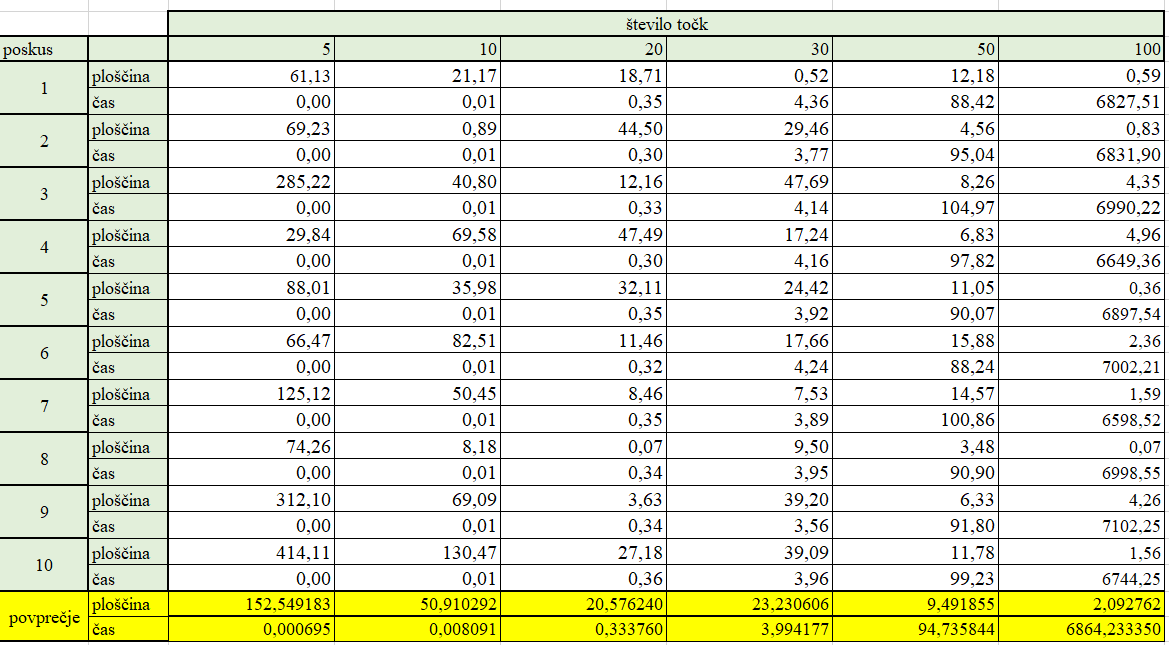
\includegraphics[width= \textwidth]{tabela}
  \caption{Tabela meritev}
\end{figure}

\begin{figure}[H]
  \centering
  \newpage
  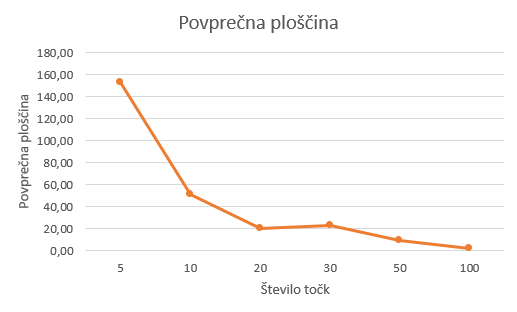
\includegraphics[width= 0.8\textwidth]{ploscina2}
  \caption{Graf povprečne ploščine za 5-100 točk}
\end{figure}

\begin{figure}[H]
  \centering
  \newpage
  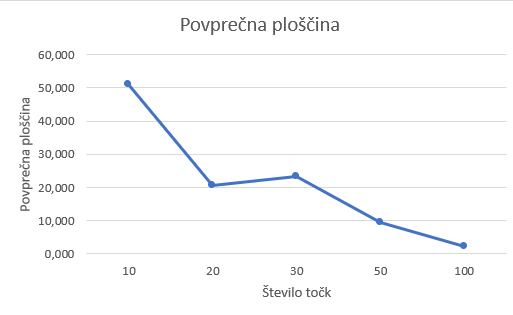
\includegraphics[width= 0.8\textwidth]{ploscina1}
  \caption{Graf povprečne ploščine za 5-50 točk}
\end{figure}

Grafa prikazujeta spreminjanje povprečne ploščine največjega večkotnika, če povečujemo število točk. V prvem grafu so vključene meritve za 5-100 točk, v drugem pa za bolj nazoren prikaz le meritve za 10-100 točk.

Ploščine se pri povečevanju točk postopoma manjšajo. Za 5 točk je ploščina povprečno enaka približno 150 kvadratnih enot, kar je približno 6\% celotne ploščine. Pri 100 točkah pa je ploščina le še povprečno približno 2 kvadratni enoti, kar je 0,08\% celotne ploščine.

\begin{figure}[H]
  \centering
  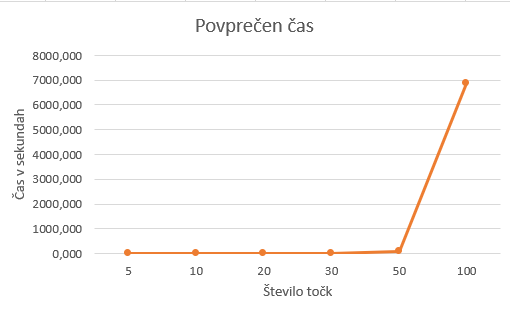
\includegraphics[width= 0.8\textwidth]{cas2}
  \caption{Graf povprečnega časa za 5-100 točk}
\end{figure}

\begin{figure}[H]
  \centering
  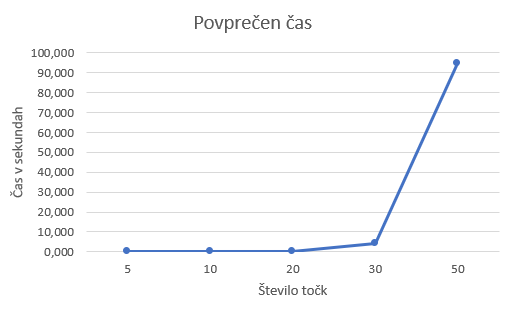
\includegraphics[width= 0.8\textwidth]{cas1}
  \caption{Graf povprečnega časa za 5-50 točk}
\end{figure}

Grafa prikazuje spreminjanje povprečnega časa, ki ga algoritem porabi za izračun največje ploščine v odvisnosti od števila točk. Tudi v tem primeru so v prvi graf vključene meritve za 5-100 točk, v drugi pa za bolj nazoren prikaz le meritve za 5-50 točk.

Algoritem učinkovito računa ploščine za 5, 10 in 20 točk. Za 30 točk še vedno potrebuje le povprečno približno 4 sekunde, medtem ko se za 50 točk čas delovanja poveča že na približno minuto in pol, za 100 točk pa kar na več kot 6500 sekund, kar je skoraj dve uri. 

Zaradi časovne zahtevnosti algoritma poskusov za večje število točk nisva izvajala.

\section{Viri}

\begin{itemize}
	\item C. Bautista-Santiagoa, J.M. Díaz-Báñez, D. Lara, P. Pérez-Lanteroc, J. Urrutia, I. Venturai: Computing optimal islands (objavljeno: april, 2011)

\end{itemize}

\end{document}

